\documentclass[10pt,a4paper,reqno]{amsart}
\usepackage[T1]{fontenc}
\usepackage{macros}
\usepackage{tikz}

\begin{document}
\bibliographystyle{alpha}

\noindent \textit{Algebraic Number Theory, Math 421}

\noindent \textit{Instructor: Sreekar M. Shastry}

\noindent \emph{Notes on the distribution of ideals in number fields} (\cite[Ch.6]{M})

\bigskip
We use the usual notation, $K, L/K, G, \OK, \OL, P, Q, \dots$

\bigskip

\begin{ap}
Roughly speaking, the idea is to show that the ideals of \OK{} are
approximately equidistributed among the ideal classes and that the number of
ideals with $\norm{I} \le t$ is approximately proportional to $t$.
\end{ap}

\begin{defn}
Write $n = [K:\Q]$ and for each $t \ge 0$ put \[i(t) := \# \{\text{ideals } I
\subset \OK : \norm{I} \le t\}\] and for $C\in \Cl{K}$, put \[i_C(t) := \#
\{\text{ideals } I \in C : \norm{I} \le t\}\] so that we have \[i(t) =
\sum_{C\in\Cl{K}} i_C(t).\] This is a finite sum since the class group is
finite.
\end{defn}

\begin{thm}
There is a number $\kappa$ depending only on \OK{} such that \[i_C(t) = \kappa
t + \varepsilon_C(t)\] where the error term is\footnote{Recall that $f = O(g)$
iff $\limsup_{x\rightarrow \infty} \left|\frac{f(x)}{g(x)}\right| < \infty$
or equivalently, $\frac{f(x)}{g(x)}$ is bounded as $x\rightarrow \infty$.}
\[\varepsilon_C(t) = O(t^{1-1/n}).\]
\end{thm}

\begin{rem}
We will determine $\kappa$ later. This theorem is a refinement of and implies
the statement \[\frac{i_C(t)}{t} \rightarrow \kappa \text{ as } t \rightarrow
\infty.\] Summing over $C$ we obtain the
\end{rem}

\begin{cor}
$i(t) = \kappa h_K t + \varepsilon(t)$ where $h_K := \# \Cl{K}$ and
$\varepsilon(t) = O(t^{1-1/n}).$
\end{cor}

\begin{rems}
(a) This corollary will lead to the class number formula.

(b) Let us note that in the case $K=\Q$, $i(t) = [t]$ is the greatest integer
$\le t$ so that $\kappa=1$ and $\varepsilon(t) = [t]-t$. The condition
$\varepsilon(t) = O(t^{1-1/n}) = O(1)$ just expresses the fact that
$\varepsilon(t)$ is bounded.
\end{rems}

\begin{proof}[Proof of the Theorem]
The idea is to count ideals in $C$ by counting elements in a certain ideal.
Let us fix an ideal $J \in C^{-1}$. Then there is a bijection
\[ \left\{
\begin{array}{c}
    \text{ideals } I \in C \\
    \text{s.t. } \norm{I} \le t
\end{array}
\right\} \longleftrightarrow
\left\{
\begin{array}{c}
    \text{principal ideals } (\alpha) \subset J \\
    \text{s.t. } \norm{(\alpha)} \le t\norm{J}
\end{array}
\right\} \] in which $I$ corresponds to $IJ = (\alpha)$. Counting principal
ideals $(\alpha) \subset J$ amounts to counting orbits of $J$ under the action
of $U := \OK^{\times}$.

(We may rephrase the above as follows. Put \[J_t := \{\alpha\in J :
\norm{(\alpha)} \le t\norm{J}\}.\] Then the $U$ action on $J$ restricts to an
action on $J_t$; the latter is a finite set because of what we know about the
geometry of numbers and we have \[i_C(t) = \#(U \backslash J_t). \] It is this
set that we shall count.)

If $K$ contained only finitely many units then we would have that $\#U .
i_C(t)$ coincides with the number of elements $\alpha \in J$ such that
$\norm{(\alpha)} \le t \norm{J}$ and we might use geometric arguments with
lattices to attack the problem.

There is one nontrivial case in which $\#U$ is finite, namely when $K$ is
imaginary quadratic. Let us consider this case first as it will give us some
insight for the general case. Thus, until further notice, $K$ is assumed to be
imaginary quadratic.

We know that $\OK$ is a lattice in \C{} and therefore so is $J$. Moreover,
$\norm{(\alpha)} = \Nm_{K/\Q}(\alpha) = |\alpha|^2$ for $\alpha\neq 0$.
Therefore we seek to count the number of nonzero elements of $J$ in the circle
of radius $\sqrt{t\norm{J}}$ centered at 0. Let $F$ be a fundamental domain for
$J \subset \C$ and consider the translates of $F$ centered at the various
points of $J$; the number of points of $J$ in a circle of radius $\rho$ is
approximately the number of these translates which are contained in the circle,
and the latter is approximately $\pi\rho^2/\vol(F).$

These estimates are good for large $\rho$; specifically, let $n^-(\rho)$ be the
number of translates of $F$ which are centered at points of $J$ and which are
entirely contained within a circle of radius $\rho$ centered at 0 and let
$n^+(\rho)$ be the number of such translates which intersect the interior of
the circle. Then, writing $n(\rho)$ for the number of points of $J$ inside the
circle, we have \[n^-(\rho) \le n(\rho) \le n^+(\rho).\]

Now, writing $\delta$ for the length of the longer diagonal of the
parallelogram $F$, we have \[n^+(\rho) \le n^-(\rho+\delta) \text{ for all }
\rho\] and thus \[n^+(\rho-\delta) \le n(\rho) \le n^-(\rho+\delta).\]
Multiplying by $\vol(F)$ we obtain \[\pi(\rho-\delta)^2 \le n(\rho) \vol(F) \le
\pi(\rho+\delta)^2.\] We have used the fact that $n^-(r)\vol(F) \le \pi r^2 \le
n^+(r)\vol(F)$. Hence $n(\rho) \vol(F) = \pi \rho^2 + \gamma(\rho)$ where
\[|\gamma(\rho)| \le \pi (2\rho\delta+\delta^2).\]

Using \[\#U . i_C(t) = n\left( \sqrt{t\norm{J}} \right) -1 \] (where the $-1$
comes from the fact that we are only counting the nonzero points of $J$; the
notation refers to the function $n(\cdot)$ defined above, not to the degree
$n=[K:\Q] =2$) we find that \[i_C(t) = \frac{\pi t\norm{J}}{\#U . \vol(F)} +
\varepsilon(t)\] with $\frac{\varepsilon(t)}{\sqrt{t}}$ bounded as
$t\rightarrow \infty$. (Verify the details.) In other words, $\varepsilon(t) =
O(\sqrt{t})$.

From what we know about the geometry of numbers\footnote{In greater detail, we
are using the facts

(i) a fundamental domain for the lattice $\iota(\OK)$ has volume
\[\frac{1}{2^s}\sqrt{|\disc{\OK}|},\] and

(ii) for a sublattice $\Lambda' \subset \Lambda$, the group $\Lambda/\Lambda'$
is finite and we have \[\vol(\R^n/\Lambda') =
\vol(\R^n/\Lambda)|\Lambda/\Lambda'|\] so that for an ideal $I \subset \OK$ we
obtain \[\vol(\R^n/\Lambda_I) =
\vol(\R^n/\Lambda_{\OK})|\Lambda_{\OK}/\Lambda_I| =
\frac{1}{2^s}(|\disc{\OK}|)^{1/2}\norm{I}\]}, we have \[\vol(F) =
\vol(\C/\OK)\norm{J} = \frac{1}{2} \norm{J} \sqrt{|\disc{\OK}}.\] Thus the
theorem holds for imaginary quadratic fields with \[\kappa = \frac{2\pi}{ \#U .
\sqrt{|\disc{\OK}|}}\] which simplifies to \[\frac{\pi}{\sqrt{|\disc{\OK}|}}\]
unless $K = \Q[i],\Q[\sqrt{-3}]$ in which case there is an extra factor of $2,$
resp.~$3$ in the denominator.

Returning to the general case\ldots

Recall that $i_C(t) = $ the number of principal ideals $(\alpha) \subset J$
with $\norm{(\alpha)} \le t\norm{J}. $ Let $S \subset \OK$ be a set of
representatives for the orbit space $U\backslash (\OK - \{0\})$. We will count
the number of elements of $J\cap S$ such that $\norm{\cdot} \le t \norm{J}$.

It will suffice to construct representatives for a free abelian subgroup $V :=
U_{\text{free}}$ of rank $r+s-1$. In other words, thus we are no longer
counting $i_C(t)$ itself, but rather the quantity obtained from the
representatives of the action on $\OK - \{0\}$ of $V$ where $U/V =
U_{\text{tors}}$ is a finite group. The proof that it is sufficient to count
w.r.t~$V$ instead of w.r.t.~$U$ will be given below.

We have the mappings \[V \subset U \subset \OK - \{0\} \rightarrow
\Lambda_{\OK} - \{0\} \xrightarrow{\log} \R^{r+s}\] from earlier. $U$ maps
onto a lattice $\Lambda_U \subset H \subset \R^{r+s}$ where $H$ is the trace
zero hyperplane. The kernel of $U\rightarrow \Lambda_U$ is the set of roots of
unity and the restriction $V \rightarrow \Lambda_U$ is an isomorphism.

Replace $\R^n$ with $\R^r\times \C^s$; recall that $n= r + 2s$. We may then
regard $\Lambda_{\OK} \subset \R^n$ as a subset of $\R^r\times \C^s$, and
thence regard $\Lambda_{\OK} \subset (\R^\times)^r\times (\C^\times)^s.$ We
extend the $\log$ map to all of $(\R^\times)^r\times (\C^\times)^s$ in the
obvious manner: \[\log(x_1,\dots,x_r,z_1,\dots,z_s) := (\log |x_1|, \dots,
2\log|z_1|,\dots).\] (The factor of 2 is to ensure compatibility with our
earlier definition of $\log$). Therefore we have \[V \subset U \subset \OK -
\{0\} \hookrightarrow (\R^\times)^r\times (\C^\times)^s \xrightarrow{\log}
\R^{r+s}.\] Moreover the map $\hookrightarrow$ is a homomorphism of groups
w.r.t~multiplication of $K$ on the source and componentwise multiplication on
the target; \[\OK - \{0\} \ni \alpha \mapsto (\sigma_1(\alpha), \dots,
\sigma_r(\alpha), \tau_1(\alpha), \dots, \tau_s(\alpha)) \in
(\R^\times)^r\times (\C^\times)^s.\] Write $V'$ for the image of $V$ in
$(\R^\times)^r\times (\C^\times)^s$.

A set of coset reps for $V$ in $\OK - \{0\}$ may be obtained from a set of
coset reps for $V'$ in $(\R^\times)^r\times (\C^\times)^s$ namely, a set of
coset reps is the same thing as a fundamental domain for $V' \subset
(\R^\times)^r\times (\C^\times)^s$. Counting elements of the ideal $J$ in the
desired subset of $\OK - \{0\}$ is therefore the same as counting elements of
the lattice $\Lambda_J$ inside the fundamental domain. Moreover the condition
\[\norm{(\alpha)} \le t \norm{J}\] is equivalent to
\[|\mathrm{N}(\overline{\alpha})| \le t\norm{J}\] where $\overline{\alpha}$ is
the image of $\alpha$ in $(\R^\times)^r\times (\C^\times)^s$ and $\mathrm{N}$
is the ``norm'' defined by \[\mathrm{N}(x_1,\dots,x_r,z_1,\dots,z_s) = x_1
\cdots x_r |z_1|^2 \cdots |z_s|^2.\] (Verify this.)

To summarize, it remains to

(1) find a set $D$ of coset reps for $V' \subset (\R^\times)^r\times
(\C^\times)^s$;

(2) count elements $x\in \Lambda_J\cap D$ s.t. \(|\mathrm{N}(x)| \le
t\norm{J}.\)

Now let us show that it suffices to work with $V = U_{\text{free}}$ instead of
all of $U$. The number of $x$ in (2) is essentially the number of principal
ideals $(\alpha)\subset J$ with $\norm{(\alpha)} \le t\norm{J}$ except that
each such ideal has been counted $w := \# U_{\text{tors}}$ times. Thus the
number of $x$ in (2) is $w. i_C(t)$.

To construct $D$ we need the following obvious Lemma whose proof is left as an
exercise.

\bigskip

\emph{Lemma A. Let $f : G'\rightarrow G$ be a homomorphism of abelian groups
and let $S'$ be a subgroup of $G'$ which is carried isomorphically onto the
subgroup $S\subset G$. Suppose that $D$ is a set of coset reps for $S \subset
G$. Then $D' := f^{-1}(D)$ is a set of coset reps for $S' \subset G'.$}

\emph{Proof of Lemma A.} This follows upon noting that, since $S'$ is carried
isomorphically onto $S$, $\ker(f)\cap S'$ is trivial. Thus we have a
bijections between $\ker(f) \times D$, $D' = f^{-1}(D)$ and $G'/S'$ which lift
the bijections between $\{1\} \times D$, $D$ and $G/S$.~///

\bigskip

We apply Lemma A to the homomorphism $\log : (\R^\times)^r\times (\C^\times)^s
\rightarrow \R^{r+s}.$\footnote{Recall the definition of log: \begin{align*}
\R^{r+2s} & \supset \Lambda_{\OK} - \{0\} \ni (x_1,\dots,x_n) \mapsto \\ &
(\log|x_1|,\dots,\log|x_r|, \underbrace{\log(x^2_{r+1}+x^2_{r+2}),\dots,
\log(x_{n-1}^2+x_n^2)}_{s} ) \in \R^{r+s}.  \end{align*} } We know that $V'$
maps isomorphically onto the lattice $\Lambda_U$ so what we seek is a set $D$
of coset reps for $\Lambda_U$ in $\R^n$; then its preimage $D'$ will be the
sought fundamental domain.

As an example, consider the real quadratic case, so that $r=2,s=0$ and
$\Lambda_U$ is a one dimensional lattice in the line $x+y=0$. $D$ can be taken
to be the half-open infinite strip shown in the diagram on the left, and its
preimage $D'$ in $(\R^\times)^2$ is shown on the right.

\begin{center}
    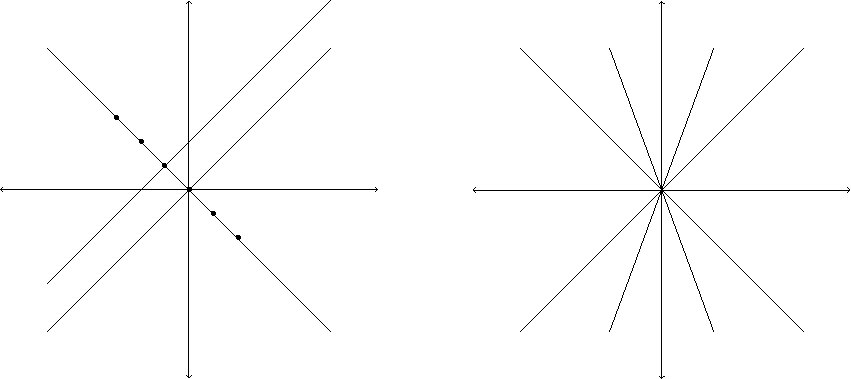
\includegraphics[scale=0.8]{resources/marcus-fund-domain}
\end{center}

In general, let $F$ be a fundamental domain $F$ for $\Lambda_U \subset H$ and
take $D$ to be the direct product $F\times \R.v$ where $\R.v$ is any line
through the origin not contained in $H$, i.e.~$v\in \R^{r+s}-H$. Then $$D' =
\{x \in (\R^\times)^r\times (\C^\times)^s : \log x \in F \times \R.v\}$$ is a
fundamental domain for $V'$.

Since we have the fundamental domain $D'$, we no longer need to keep track of
what we called $D$ above, and therefore to ease notation we will write $D = D'$
henceforth.

The best choice of $v$ will turn out to be \[v_0 :=
(\underbrace{1,\dots,1}_{r},\underbrace{2,\dots,2}_{s}).\] (In the real
quadratic case, $v_0 = (1,1)$.) With this choice of $v=v_0$, we have $D=aD$ for
all $a\in \R-\{0\}$. (Verify this.)

Recall that we sought to count the number of points $x$ in $\Lambda_J\cap D$
s.t.~$|\mathrm{N}(x)| \le t\norm{J}.$ For this purpose we define \[D_a :=
\{x\in D: |\mathrm{N}(x)| \le a\}\] and note that we have \[D_a = a^{1/n}
D_1.\] Thus we have reduced to counting the number of points in \[\Lambda_J\cap
(t\norm{J})^{1/n}D_1.\] More precisely, we want an asymptotic estimate for this
number as $t\rightarrow \infty.$

We will obtain such an estimate under rather general conditions. Let $\Lambda$
be a lattice in $\R^n$ and let $B$ be any bounded subset of $\R^n$. We seek to
estimate $|\Lambda\cap aB|$ as $a\rightarrow \infty.$

\bigskip

\emph{Lemma B. If $B$ has a sufficiently nice boundary (to be made precise
later) then \[|\Lambda\cap aB| = \frac{\vol(B)}{\vol(\R^n/\Lambda)}a^n +
\gamma(a)\] where $\gamma(a) = O(a^{n-1})$.}

\bigskip

To apply this we consider $(\R^\times)^r\times (\C^\times)^s$ to be contained
in $\R^n$ in the obvious manner. Grant for the moment that $D_1$ is bounded and
has sufficiently nice boundary. Then we obtain \[|\Lambda_J \cap
(t\norm{J})^{1/n}D_1 | = \frac{\vol(D_1)\norm{J}}{\vol(\R^n/\Lambda_J)}t +
\delta(t)\] where $\delta(t) = O(t^{1-1/n}).$ The coefficient of $t$ simplifies
to \[\frac{\vol(D_1)}{\vol(\R^n/\Lambda_{\OK})}.\] Thus we finally obtain
\[i_C(t) = \kappa t + \varepsilon(t)\] with $\varepsilon(t) = O(t^{1-1/n})$ and
\[\kappa = \frac{\vol(D_1)}{w.\vol(\R^n/\Lambda_{\OK})} = \frac{2^s \vol(D_1)}{
w|\disc{\OK}|^{1/2}}.\]

The proof will be complete after we

(a) define ``sufficiently nice''

(b) prove Lemma B

(c) show that $D_1$ is bounded and has a sufficiently nice boundary

We do not need $\vol(D_1)$ for the proof of the theorem, but we will compute it
later since it will lead to the class number formula.

\bigskip

``Sufficiently nice boundary'' means $(n-1)$-Lipschitz parametrizable. This
means that the boundary is covered by the images of finitely many Lipschitz
functions $f : [0,1]^{n-1} \rightarrow \R^n$; the condition is that the ratio
\[\frac{|f(x)-f(y)|}{|x-y|}\] is bounded as $x,y$ range over $[0,1]^{n-1}$ and
$|\cdot|$ is the metric in $\R^n,\R^{n-1}$ as appropriate.

\emph{Proof of Lemma B.} Let us reduce the problem to $\Lambda = \Z^n.$ Take
$\varphi\in GL_n(\R)$ which carries $\Lambda$ to $\Z^n.$ Since the Lipschitz
condition is preserved by linear transformations, we have that $B' =
\varphi(B)$ has a sufficiently nice boundary. Clearly \[|\Lambda\cap aB| = |
\Z^n\cap aB'|\] so that it will suffice to show that the Lemma holds for $\Z^n$
and that \[\vol(B') = \frac{\vol(B)}{\vol(\R^n/\Lambda)}.\] The latter
assertion follows from the calculation
\[\frac{\vol(\R^n/\Lambda)}{\vol(\R^n/\Z^n)} = \frac{\vol(B)}{\vol(B')} =
|\det(\varphi)|.\] This equation expresses the effect of a linear
transformation on Lebesgue measure, namely that all volumes are scaled by the
determinant. Noting that $\vol(\R^n/\Z^n) = 1$ gives the sought equality.

Thus we take $\Lambda = \Z^n.$ Consider the translates of the unit cube
$[0,1]^n$ centered at points of $\Z^n$. We will call any such translate a cube.
The number of cubes inside $aB$ is approximately $|\Z^n\cap aB|$ and likewise
approximately $\vol(aB).$ In either case, the difference between the actual
count of cubes and the approximate value is bounded by the number of cubes
which meet the boundary of $aB.$ Hence it will suffice to show that this last
number is $O(a^{n-1})$ for then it will follow that \[|\Z^n \cap aB | =
\vol(aB) + \gamma(a) = a^n\vol(B) + \gamma(a)\] with $\gamma(a) = O(a^{n-1})$.
This will complete the proof of Lemma B for $\Z^n$.

$\partial B$ is covered by the sets $f([0,1]^{n-1})$ for finitely many
Lipschitz functions $f$ and thus the boundary of $aB$ is covered by the sets
\[a.f([0,1]^{n-1}).\] Fixing one such $f$, it is enough to show that the number
of cubes intersecting $a.f([0,1]^{n-1})$ is $O(a^{n-1})$. (This is in a way a
geometrically obvious statement. The scale by $a$ would produce the factor of
$a^{n-1}$ and the Lipschitz property produces a constant which is subsumed by
the $O$-notation.)

We subdivide $[0,1]^{n-1}$ into $[a]^{n-1}$ smaller cubes in the obvious
manner, where $[a]$ is the greatest integer $\le a.$ Without loss, $a \ge 1$
(we are interested in the asymptotics as $a\rightarrow \infty$). Each small
cube $S$ has diagonal $\sqrt{n-1}/[a]$ so that the diameter of $f(S)$ is at
most $\lambda\sqrt{n-1}/[a]$ where $\lambda$ is the Lipschitz bound for $f$.
Then $a.f(S)$ has diameter at most $a\lambda\sqrt{n-1}/[a]$; this is at most
$2\lambda\sqrt{n-1}$ since $a\ge 1$. Crucially, note that this last quantity,
$2\lambda\sqrt{n-1}$, is independent of $a$.

We now make a gross estimate. Fix a point $x\in a.f(S)$ and take the open
$n$-ball centered at that point of radius $2\lambda\sqrt{n-1}$,
$B_x(2\lambda\sqrt{n-1}) \subset \R^n$. It is clear that this ball contains
$a.f(S)$ and intersects at most \[\mu = (4\lambda\sqrt{n-1}+2)^n\] cubes. Note
that $\mu$ is independent of $a$. It follows that the number of cubes
intersecting $a.f([0,1]^{n-1})$ is at most $\mu[a]^{n-1}$ since $[0,1]^{n-1} =
$ the union of $[a]^{n-1}$ translates of the small cube $S$. Finally, to
complete the proof of the lemma, we have \[\mu[a]^{n-1} = O(a^{n-1}),\] as
required. ///

We have dispensed with (a) and (b) above. Now we must attend to (c) by showing
that $D_1$ is bounded and has a sufficiently nice boundary.

Recall that $D_1$ consists of all $x = (x_1,\dots,x_r,z_1,\dots,z_s) \in
(\R^\times)^r \times (\C^\times)^s$ s.t. \[\log(x) = (\log|x_1| , \dots,
2\log|z_1| , \dots) \in F\oplus \R.v_0\] and s.t.~$|x_1\cdots x_r z_1^2 \cdots
z_s^2| \le 1.$ This last condition is equivalent to saying that $\log(x)$ has
coordinate sum $\le 0.$ It follows that \[x\in D_1 \text{ iff } \log(x) \in F
\times (-\infty,0].v_0.\]

Using this let us see that $D_1$ is bounded: the fact that $F$ is bounded
places bounds on all coordinates of points of $F$ and therefore the coordinates
of the points of $F \times (-\infty,0].v_0$ are bounded above. The points of
$D_1$ are thus bounded by definition of $\log$ (namely, $\log^{-1}= \exp$ of a
negative number is in $[0,1]$). Thus $D_1 \subset (\R^\times)^r \times
(\C^\times)^s $ is bounded.

This is what $D_1$ looks like in the real quadratic case.

\begin{center}
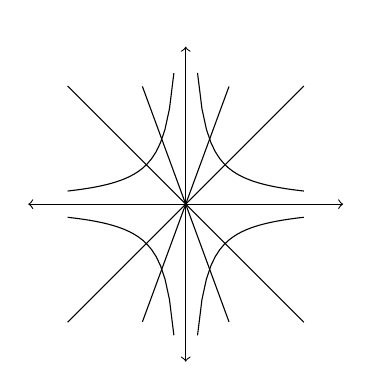
\begin{tikzpicture}[domain=-4:4,scale=0.5]
\draw[<->] (-4,0) -- (4,0) node[right] {};
\draw[<->] (0,-4) -- (0,4) node[above] {};
\draw[domain=-3:3]   plot (\x,\x)    node[right] {};
\draw[domain=-3:3]   plot (\x,-\x)   node[right] {};
\draw[domain=-1.1:1.1]   plot (\x,2.71828*\x)    node[right] {};
\draw[domain=-1.1:1.1]   plot (\x,-2.71828*\x)   node[right] {};
\draw[domain=-3:-0.3]   plot (\x,1/\x)   node[right] {};
\draw[domain=-3:-0.3]   plot (\x,-1/\x)   node[right] {};
\draw[domain=0.3:3]   plot (\x,1/\x)   node[right] {};
\draw[domain=0.3:3]   plot (\x,-1/\x)   node[right] {};
\end{tikzpicture}
\end{center}

From the figure, it is clear that the boundary of $D_1$ is 1-Lipschitz
parametrizable, so the proof is complete for real quadratic fields.

Returning to the general case, we replace $D_1$ with the subset $D_1^+$
consisting of the points s.t.~$x_1 \ge 0, \dots, x_r \ge 0.$ $D_1$ has a
sufficiently nice boundary iff $D_1^+$ does and $\vol(D_1) = 2^r \vol(D_1^+)$
(in other words, to make $D_1^+$ we are choosing half of each real coordinate
of $D_1$).

Let us construct a Lipschitz parametrization of $\partial D_1^+.$ We need some
notation. The fundamental domain $F$ is of the form \[\left\{
\sum_{k=1}^{r+s-1} t_k v_k : 0 \le t_k \le 1 \right\}\] where
$\{v_1,\dots,v_{r+s-1}\}$ is a $\Z$-basis for the lattice $\Lambda_U.$ For each
$k$, write \[v_k = (v^1_k,\dots,v^{r+s}_k)\] (recall that $v_k \in \Lambda_U
\subset H \subset \R^{r+s}$; $H$ is the trace zero hyperplane in $\R^{r+s}$,
not $\R^{r+2s}$). A point $(x_1,\dots,x_r,z_1,\dots,z_s)\in D_1^+$ is
characterized by the equations
\begin{align*}
\log(x_j)       &= \sum_{k=1}^{r+s-1} t_k v_r^j + u & 1 \le j \le r \\
2 \log|z_j|     &= \sum_{k=1}^{r+s-1} t_k v_r^j + 2u & r+1 \le j \le r+s.
\end{align*} Here, $x_j > 0, t_k \in [0,1), u\in (-\infty, 0]$. Write $t_{r+s}
= e^u$ and introduce polar coordinates $(\rho_j,\theta_j)$ for each $z_j$ so
that we may write $D_1^+$ as the set of $$(x_1,\dots,x_r,\rho_1
e^{i\theta_1},\dots, \rho_s e^{i\theta_s})$$ s.t.
\begin{align*}
x_j & = t_{r+s}\exp\left\{\sum_{k=1}^{r+s-1} t_k v_k^j \right\} \\
\rho_j &= t_{r+s} \exp\left\{ \frac{1}{2} \sum_{k=1}^{r+s-1} t_k
v_k^{r+j} \right\} \\
\theta_j & = 2\pi t_{r+s+j}
\end{align*} with $t_{r+s} \in (0,1]$ and the other $t_k\in [0,1)$. This gives
a parametrization of $D_1^+$ by a half-open $n$-cube. Letting all the $t_k$
take on their boundary values, we obtain a parametrization of the closure
$\overline{D_1^+}$. In other words, we have a function \[f : [0,1]^n
\rightarrow \R^r\times \C^s\] mapping the cube onto $\overline{D_1^+}$. (To
prove that the image is $\overline{D_1^+}$, note that since $[0,1]^n$ is
compact and $f$ is continuous, the image is a compact hence closed set
containing $D_1^+$. On the other hand, the half open cube is dense in the cube,
hence $D_1^+$ is dense in the image. Therefore the image is exactly
$\overline{D_1^+}$.)

The closure $\overline{D_1^+}$ is the disjoint union of the interior $I$ and
the boundary $B := \partial \overline{D_1^+}$. We shall show that the interior
of the cube is sent to $I$ and hence that the boundary of the cube is mapped
onto a set containing $B$. The boundary of the cube is the union of $2n$
$(n-1)$-cubes, hence $B$ is covered by the images of the $2n$ mappings from
$(n-1)$-cubes. Each of these mappings is Lipschitz because $f$ is (a fact which
we will prove below) and hence $B$ is $(n-1)$-Lipschitz parametrizable. This is
what we had to show.

It remains to prove that $f$ is Lipschitz and that the interior $(0,1)^n
\subset [0,1]^n$ is mapped into the interior $I$ of $D_1^+.$

To show that $f$ is Lipschitz, note that all of its partial derivatives exist
and are continuous and therefore all partial derivatives are bounded on
$[0,1]^n$ (a continuous function on a compact set is bounded). This implies
that $f$ is Lipschitz (note well the intervention of the polar coordinates
$\rho_j, \theta_j.$)

Finally, we must show that $(0,1)^n$ is sent to $I$. We claim that the
restriction \[f: (0,1)^n \rightarrow \R^r\times \C^s\] is the composite of four
maps \[(0,1)^n \xrightarrow{f_1} \R^n \xrightarrow{f_2} \R^n \xrightarrow{f_3}
\R^r\times (0,\infty)^s \times \R^s \xrightarrow{f_4} \R^r\times \C^s\] each
of which preseves open sets. Granting this assertion, it follows that
$(0,1)^n$ is mapped onto an open set by $f$ and therefore is sent into $I$.

The $f_i$ are defined as follows. \[f_1(t_1,\dots,t_n) := (t_1,
\dots,\log(t_{r+s}), \dots,t_n),\] where the log is applied only to the
$(r+s)$th coordinate. $f_2$ is the linear transformation \[f_2(u_1,\dots,u_n)
:= (u_1,\dots,u_n)M \] where $M$ is the $n\times n$ matrix
\begin{center}
    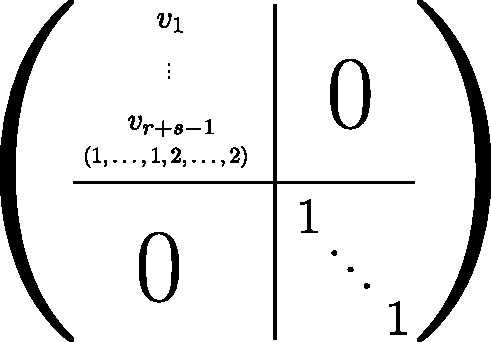
\includegraphics[scale=0.8]{resources/marcus-ch6-mtx}
\end{center}

$f_3$ is defined by applying the function $e^x$ to each of the first $r$ (real,
rectangular) coordinates $x$; applying $\frac{1}{2}e^x$ to each of the next $s$
(radial) coordinates; multiplying each of the last $s$ (angular) coordinates by
$2\pi.$

Finally $f_4$ sends \[(x_1,\dots,x_r,\rho_1,\dots,\rho_s,
\theta_1,\dots,\theta_s)\] to \[ (x_1,\dots,x_r,\rho_1 e^{i\theta_1},\dots,
\rho_s e^{i\theta_s}) \in \R^r\times \C^s. \] One checks that $f = f_1 ; f_2 ;
f_3 ; f_4$. (Please do so!) Now, $f_1,f_3,f_4$ are defined in terms of
$\log,\exp,$ and scalar multiplication, each of which are local
diffeomorphisms, and therefore $f_1,f_3,f_4$ take open sets to open sets. It
remains to prove that the linear transformation $f_2$ takes open sets to open
sets, or in other words, that it has rank $n$. This is clear from the shape of
the matrix since since the $v_k$ and $v_0 := (1,\dots,1,2,\dots,2)$ are
linearly independent in $\R^{r+s}.$ (Recall that $\{v_i\}$ is a \Z-basis for a
lattice contained in the trace zero hyperplane; (1,\dots,1,2,\dots,2) is not in
this hyperplane.)

This completes the proof of the theorem.
\end{proof}

\begin{ap}
Our next objective is to give a formula for $\kappa.$ This requires that we
calculate \[\vol(D_1) = 2^r \vol(D_1^+).\] In polar coordinates, we have
\[\vol(D_1^+) = \int_{D_1^+} \rho_1 \cdots \rho_s dx_1 \cdots dx_r d\rho_1
\cdots d\rho_s d\theta_1 \cdots d\theta_s\] (we may figuratively write
$\vol(D_1^+) = \int_{D_1^+} \rho\ dx\ d\rho\ d\theta.$)

Changing coordinates, this integral becomes \[\int_{[0,1]^n} \rho_1 \cdots
\rho_s |J(t_1,\dots,t_n)| dt_1 \cdots dt_n\] where $J$ is the Jacobian matrix
of $f$. $J$ is the matrix having as its entries the partial derivatives of the
functions $x_j,\rho_j,\theta_j$ w.r.t.~$t_k.$ If we write \[w_1,\dots,w_n :=
x_1,\dots,x_r,\rho_1,\dots,\rho_s,\theta_1,\dots,\theta_s\] then we have $J =
(a_{jk})$ with \[a_{jk} = \frac{\partial w_j}{ \partial t_k}.\] (There is a
typo in \cite{M} at this point\dots)

We have, for $k < r+s$,
\begin{align*}
\frac{\partial w_j}{
\partial t_k} & = \begin{cases}
    v_k^j w_j & j \le r \\
    \frac{1}{2} v_k^j w_j & r < j \le r+s \\
    0 & j > r+s
\end{cases} \\
\frac{\partial w_j}{
\partial t_{r+s}} & = \begin{cases}
    w_j/t_{r+s} & j \le r+s\\
    0 & j > r+s
\end{cases}
\end{align*}
and for $k > r+s,$
\[ \frac{\partial w_j}{
\partial t_{k}} = \begin{cases}
    2\pi & j = k\\
    0 & \text{otherwise}.
\end{cases}\] One must verify these computations (please do so!) and check that
the determinant is given by \[\det J = \frac{\pi^s x_1 \cdots x_r \rho_1 \cdots
\rho_s}{t_{r+s}} \det(M)\] where $M$ is the matrix from the proof of the
previous theorem. Thus we obtain \[\vol(D_1^+) = \pi^s |\det(M)| \int_{[0,1]^n}
\frac{x_1 \cdots x_r \rho_1^2 \cdots \rho_s^2}{t_{r+s}} dt_1 \cdots dt_n.\]
Using the expressions for the parametrization, we have \[x_1 \cdots x_r
\rho_1^2 \cdots \rho_s^2 = t_{r+s}^n.\] In greater detail, we have
\begin{align*}
    x_1 \cdots x_r \rho_1^2 \cdots \rho_s^2 & = \prod_{j=1}^r
    t_{r+s}\exp\left\{\sum_{k=1}^{r+s-1} t_k v_k^j  \right\} \times
    \prod_{j=1}^s
    \left[
    t_{r+s}\exp\left\{\frac{1}{2}\sum_{k=1}^{r+s-1}t_k v_k^{r+j}\right\}
    \right]^2 \\
    & = t_{r+s}^{r+2s} \exp\left\{
    \sum_{k=1}^{r+s-1} t_k v_k^j +
    \sum_{k=1}^{r+s-1}t_k v_k^{r+j}
    \right\}\\
    & = t_{r+s}^n
\end{align*} because $r+2s = n$ and the $v_k$ are in the trace zero hyperplane.
Therefore \[ \vol(D_1^+) = \pi^s | \det(M) | \int_{[0,1]^n} t_{r+s}^{n-1} dt_1
\cdots dt_n = \frac{1}{n} \pi^s |\det(M)|.\]

The quantity \[\frac{1}{n} |\det(M)|\] is called the \emph{regulator} of $K$,
written as \reg{K}. In fact, the regulator is equal to the absolute value of
the determinant of the $(r+s)\times(r+s)$ matrix having as its first $r+s-1$
rows $v_1,\dots,v_{r+s-1}$ = the log vectors of a fundamental system of units
and having for its final row the vector $\frac{1}{n} (1,\dots,1,2,\dots,2).$
This quantity does not depend on the choice of basis $\{v_i\}$ (which we will
see later on). Thus \[\vol(D_1) = 2^r\pi^s\reg{K}.\] We have proven
\end{ap}

\begin{thm}
\[\kappa = \frac{2^{r+s}\pi^s \reg{K}}{w|\disc{K}|^{1/2}}\] where $r$ is the
number of real embeddings of $K$, $s$ is half the number of non-real embeddings
of $K$, and $w$ is the number of roots of unity in $K$.
\end{thm}

Let us give another characterization of the regulator. For this we will need
the following lemma.

\begin{lem}
Let $A$ be a square matrix, all of whose row sums are zero, except for the last
row. Then the determinant of $A$ is unchanged upon replacing the last row by
any other vector with the same coordinate sum.
\end{lem}

\begin{proof}
Let $B$ be the new matrix. Write $v_A,v_B$ for the last row vector of $A,B$.
Write $C$ for the matrix whose last row is $v_A - v_B$, but which is otherwise
the same as $A$ and $B$. Then we have \[\det(A) - \det(B) = \det(C).\] But the
columns of $C$ add up to the zero vector, thus the columns of $C$ are linearly
dependent, and therefore $\det(C) = 0$.
\end{proof}

Recall that $\reg{K}$ is the absolute value of the determinant of the matrix
with $v_1,\dots,v_{r+s-1}$ in its first $r+s-1$ rows and \[
(\underbrace{1/n,\dots,1/n}_{r},\underbrace{2/n,\dots,2/n}_{s}) \] in its last
row. The $v_i$ are all in the trace zero hyperplane $H$, so that the last row
may be replaced by any vector having coordinate sum 1 without affecting the
regulator (recall that $r+2s=n$). There are several candidates for the last
row. If we put 1 in one entry and 0 in the others we see that $\reg{K}$ is the
absolute value of an $(r+s-1)\times(r+s-1)$ subdeterminant. If we put $1/(r+s)$
everywhere along the last row we obtain a geometric intepretation.

\begin{thm}
\[\reg{K} = \frac{\vol(H/\Lambda_U)}{\sqrt{r+s}}\] where $\Lambda_U$ is the
lattice associated to the unit group $U \subset \OK-\{0\}$; moreover, if
$v_1,\dots,v_{r+s-1}$ is any \Z-basis for $\Lambda_U$ then \reg{K} is the
absolute value of the determinant obtained by deleting any column from the
matrix with rows $v_1,\dots,v_{r+s-1}$.
\end{thm}

\begin{proof}
Let $\Lambda$ be the lattice in $\R^{r+s}$ with \Z-basis
\[\left\{v_1,\dots,v_{r+s-1},\left( \frac{1}{r+s},\dots,\frac{1}{r+s} \right)
\right\}.\] Then by the lemma and the above discussion and what we know about
the relationship between volumes and determinants, we have \[\reg{K} =
\vol(\R^{r+s}/\Lambda).\] Since the last basis vector is orthogonal to $H$ we
find that $\vol(\R^{r+s}/\Lambda)$ is the product of $\vol(H/\Lambda_U)$ and
the length of $(1/(r+s),\dots,1/(r+s)).$ This length is $(r+s)^{-1/2}.$

Incidentally, this formula shows that $\reg{K}$ is independent of the choice of
basis \Z-basis $\{v_i\}_{i=1}^{r+s-1}.$

The second statement follows by taking the last row vector to have 1 in one
coordinate and 0 in the other coordinates, applying the Lemma, and expanding
the determinant.
\end{proof}

\begin{rem}
We remind the reader that a \Z-basis for $\Lambda_U$ is gotten by taking the
log vectors of any fundamental system of units of $\OK$.
\end{rem}

\begin{eg}
Suppose that $K$ is real quadratic and let $u$ be \emph{the} fundamental unit
in \OK (\emph{the} indicates that we choose the uniquely determined $u$
s.t.~$u>1$). Then \[\reg{K} = \log u\] where the vector $\log u$ reduces in
this case to the log of a real number. Since $u>1$, no absolute values are
required. By the above, we have \[\kappa = \frac{2\log u}{\sqrt{\disc{\OK}}}.\]
(See \cite[p.33]{M} for the discriminant of a quadratic field, which in
particular tells us that the discriminant of a real quadratic field is always
positive.) In the imaginary quadratic case, we must \emph{define} \reg{K} to be
1. Then the earlier theorem gives the correct value of $\kappa.$
\end{eg}

\bibliography{bib}
\end{document}
